	\chapter{First Approach with Pandora}

In this chapter it will explained how to run for the first time Pandora from a computer.

	\section{Run Pandora Blind} \label{sssec:pandora_blind}

In this part it is explained how to run for the first time Pandora using LArSoft and enabling the visualisation of the Pandora interface.  

\subsection{UBOONECODE}  \label{sssec:uboonecode}
As very first thing, the terminal must be opened. Digit then the following comand:

\begin{verbatim}
source /cvmfs/uboone.opensciencegrid.org/products/setup_uboone.sh
setup uboonecode v06_48_00 -q e14:prof
\end{verbatim}

The first command tells the computer to go to the CERN Virtual Machine File System (cvmfs) and to look for the setup file. This .sh file contains a certain amount of instruction for your computer and it has to be used everytime a new terminal is opened. The second command tells the computer which version of uboonecode has to be used. v06${\_}$48${\_}$00 is the current version as this notes are written but it is better always to check which is the latest version. Note that both command must be typed everytime a new terminal is opened. For further details about source files see Section \ref{sssec:setup}. Then type 

\begin{verbatim}

ls $UBOONECODE_DIR/job
cp $UBOONECODE_DIR/job/reco_uboone_mcc7_driver_stage2.fcl ./myreco_uboone_mcc7_driver_stage2.fcl

\end{verbatim}

The first command shows which files are contained in the directory ${\$}$UBOONECODE${\_}$DIR/job. It is worth knowing that the dollar symbol in front of UBOONECODE${\_}$DIR is an identifier, that means the name given to a certain path to a certain folder/file. Digiting

\begin{verbatim}

echo $UBOONECODE_DIR

\end{verbatim}

gives us the path to the folder, which in this case is

\begin{verbatim}

/cvmfs/uboone.opensciencegrid.org/products/uboonecode/v06_48_00

\end{verbatim}

The second command copies from the folder in the cvmfs the file .fcl on the local machine, changing the name of the copied file in myreco${\_}$uboone${\_}$mcc7${\_}$driver${\_}$stage2. 

%\begin{figure}[h]
%\scalebox{2}{\includegraphics[width=0.5\textwidth]{/home/stefano/Documents/fermilab/thesis/pictures/excitation}}
%\centering
%\caption{Schematic view of self-trapped exciton luminescence and recombination luminescence. They both produce scintillation light.}
%\label{fig:excitation}
%\end{figure}


	\subsection{FCL files}  \label{sssec:fcl_xml}

Fermilab Hierarchical Configuration Language (FHiCL or shortered FCL) is a language created at Fermi National Accelerator Laboratory (FNAL or Fermilab). For the pourpose of this guide, only few details will be given. For a proper introduction see \cite{fcl_guide}. Conceptually, the .fcl gives a list of instructions to the LArSoft software (\cite{larsoft}). Opening the .fcl file the file is this:

\begin{verbatim}

#include "reco_uboone_mcc7_driver_common.fcl"

process_name: McRecoAprStage2

services.DetectorClocksService.InheritClockConfig:  false

services.TFileService.fileName: "reco_stage_2_hist.root"
physics.reco: [ @sequence::microboone_reco_mcc7_stage2 ]
physics.trigger_paths: [ reco ]
outputs.out1.fileName: "%ifb_%tc_reco2.root"
outputs.out1.dataTier: "reconstructed"
source.inputCommands: ["keep *_*_*_*", "drop *_*_*_McRecoStage2" ]

\end{verbatim}

At this point, rename the process name at the second line as follow:

\begin{verbatim}

process_name: PandoraWorkshop

\end{verbatim}

After that, you can try to run LArSoft for the first time. Digit

\begin{verbatim}

lar -c myreco_uboone_mcc7_driver_stage2.fcl -n 5 /path/to/reco2/file.root 

\end{verbatim}

lar -c myreco${\_}$uboone${\_}$mcc7${\_}$driver${\_}$stage2.fcl launches the LArsoft using instructions given by the .fcl file. lar indicates that you want to run LArSoft, -c that you use the following .fcl file and -n 5 indicates to do certain processes looping on the first 5 events of the .root file and /path/to/reco2/file.root is the .root file you want to open and use. It does not indicate a specific file but rather any kind of .root file related to neutrino interaction in LAr you may have. A typical starting point is 

\begin{verbatim}

/pnfs/uboone/scratch/users/uboonepro/mcc7/v05_08_00/reco2/prodgenie_bnb_nu_uboone

\end{verbatim}

or, on Cambridge HEP systems

\begin{verbatim}

/r05/dune/mcproduction_v05_08_00/larsoft_output_reco2_bnb_nu/

\end{verbatim}

Any of the root files contained in those folders is good. Reco2 means the reconstruction has come to a further stage (hard reconstruction) whilst reco1 means a primary stage of reconstruction (low reconstruction). At the end of this process, a new .root file reco${\_}$stage${\_}$2${\_}$hist.root has been created with all the data related to the reconstructed events.  To visualize the reconstruced events with pandora software we need another piece, the .xml file. 

\subsection{XML files and Enable Visualisation}  \label{sssec:xml}  

Extensible Markup Language (XML) is a language used to give a set of rules in human and machine-readable format. Digit 

\begin{verbatim}

cp $UBOONECODE_DIR/scripts/PandoraSettings_MicroBooNE_Neutrino.xml ./MyPandoraSettings_MicroBooNE_Neutrino.xml

\end{verbatim}

to copy on your local machine the .xml file from the Uboonecode directory. The .xml will be the following:

\begin{lstlisting}[language=XML, caption=Python example]

<!-- Pandora settings xml file -->

<pandora>
    <!-- GLOBAL SETTINGS -->
    <IsMonitoringEnabled>false</IsMonitoringEnabled>
    <ShouldDisplayAlgorithmInfo>false</ShouldDisplayAlgorithmInfo>
    <SingleHitTypeClusteringMode>true</SingleHitTypeClusteringMode>

    <!-- PLUGIN SETTINGS -->
    <MuonPlugin>LArMuonId</MuonPlugin>

    <!-- ALGORITHM SETTINGS -->

    <!-- NEUTRINO-INDUCED EVENT RECONSTRUCTION -->
    <algorithm type = "LArListPreparation">
        <OnlyAvailableCaloHits>true</OnlyAvailableCaloHits>
        <OutputCaloHitListNameW>CaloHitListW</OutputCaloHitListNameW>
        <OutputCaloHitListNameU>CaloHitListU</OutputCaloHitListNameU>
        <OutputCaloHitListNameV>CaloHitListV</OutputCaloHitListNameV>
        <FilteredCaloHitListName>CaloHitList2D</FilteredCaloHitListName>
        <CurrentCaloHitListReplacement>CaloHitList2D</CurrentCaloHitListReplacement>
        <OutputMCParticleListNameU>MCParticleListU</OutputMCParticleListNameU>
        <OutputMCParticleListNameV>MCParticleListV</OutputMCParticleListNameV>
        <OutputMCParticleListNameW>MCParticleListW</OutputMCParticleListNameW>
        <OutputMCParticleListName3D>MCParticleList3D</OutputMCParticleListName3D>
        <CurrentMCParticleListReplacement>MCParticleList3D</CurrentMCParticleListReplacement>
        <MipEquivalentCut>0.</MipEquivalentCut>
    </algorithm>

    <algorithm type = "LArVisualMonitoring">
        <CaloHitListNames>CaloHitListW CaloHitListU CaloHitListV</CaloHitListNames>
    </algorithm>

...

\end{lstlisting}

and then modify the first lines as it follows:

\begin{lstlisting}[language=XML, caption=Python example]

<!-- Pandora settings xml file -->

<pandora>
    <!-- GLOBAL SETTINGS -->
    <IsMonitoringEnabled>true</IsMonitoringEnabled>
    <ShouldDisplayAlgorithmInfo>true</ShouldDisplayAlgorithmInfo>
    <SingleHitTypeClusteringMode>true</SingleHitTypeClusteringMode>

...

\end{lstlisting}

This will enable the visualisation. Now go back to the .fcl file and modify it adding the .xml file and enabling PandoraNu:

\begin{lstlisting}[language=C++, caption=Python example]

#include "reco_uboone_mcc7_driver_common.fcl"

process_name: PandoraWorkshop

#services.RottGraphicsEnablingService: {}

services.DetectorClocksService.InheritClockConfig:  false

services.TFileService.fileName: "reco_stage_2_hist.root"

physics.producers.pandoraWriter: @local::microboone_pandorawriter
physics.producers.pandoraWriter.HitFinderModuleLabel: "gaushit"
physics.producers.pandoraWriter.ConfigFile: "MyPandoraSettings_Write.xml"
physics.producers.pandoraNu.HitFinderModuleLabel: "gaushit"
physics.producers.pandoraNu.ConfigFile: "MyPandoraSettings_MicroBooNE_Neutrino.xml"

physics.reco: [ pandoraNu ]
physics.trigger_paths: [ reco ]
outputs.out1.fileName: "%ifb_%tc_reco2.root"
outputs.out1.dataTier: "reconstructed"
source.inputCommands: ["keep *_*_*_*", "drop *_*_*_McRecoStage2" ]

\end{lstlisting}

We use PandoraNu because it is the part of Pandora software used for reconstruction of neutrino events. Finally, with again the command

\begin{verbatim}

lar -c myreco_uboone_mcc7_driver_stage2.fcl -n 5 /path/to/reco2/file.root 

\end{verbatim}

the pandora interacting window will appear and man should be able to visualise the reconstructed events. 

\subsection{Pandora Interface}  \label{sssec:pandora_inter} 

At this stage, giving a comprehensive explanation of the interface is not worth it. Anyways, it is important to see that the user can controll manually which stage of the reconstruction she want to see. Launching the programm the first time gives the first stage of reconstruction (see Fig. \ref{fig:pandora}), whilst after pressing for the second time enter a further stage of reconstruction will be added (see Fig. \ref{fig:pandora2}).

\begin{figure}[h]
\scalebox{1}{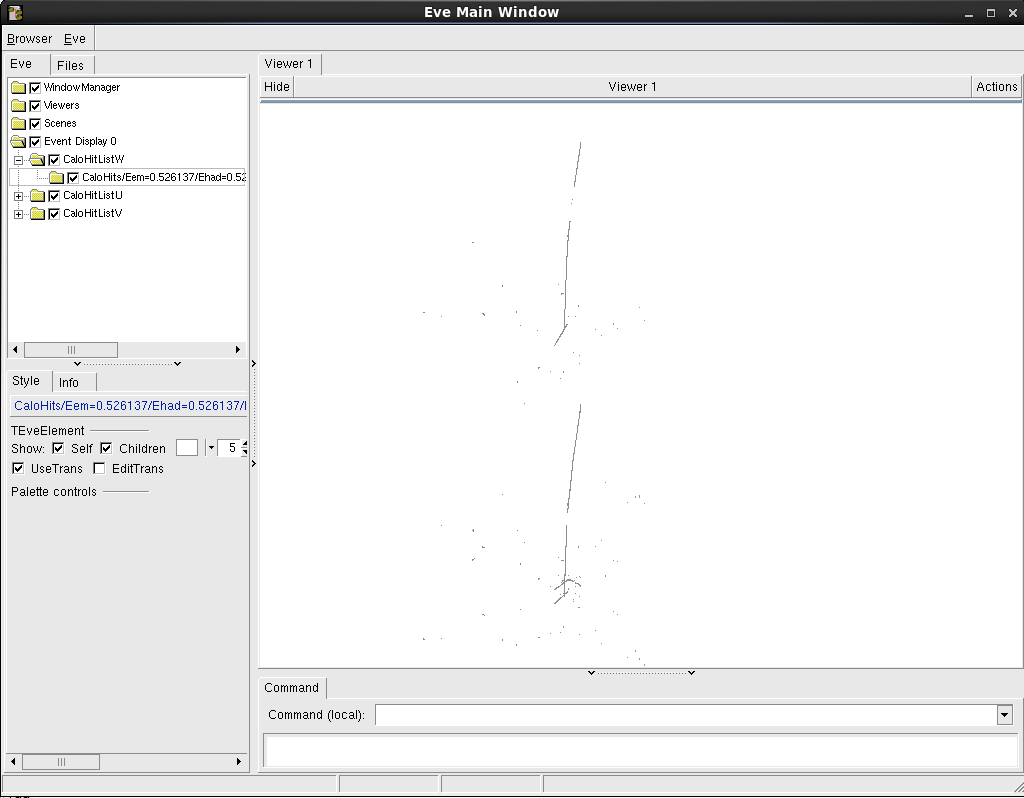
\includegraphics[width=0.5\textwidth]{/var/clus/usera/sv408/pandora_script/pandora}}
\centering
\caption{Pandora interface at first stage of reconstruction}
\label{fig:pandora}
\end{figure}

\begin{figure}[h]
\scalebox{1}{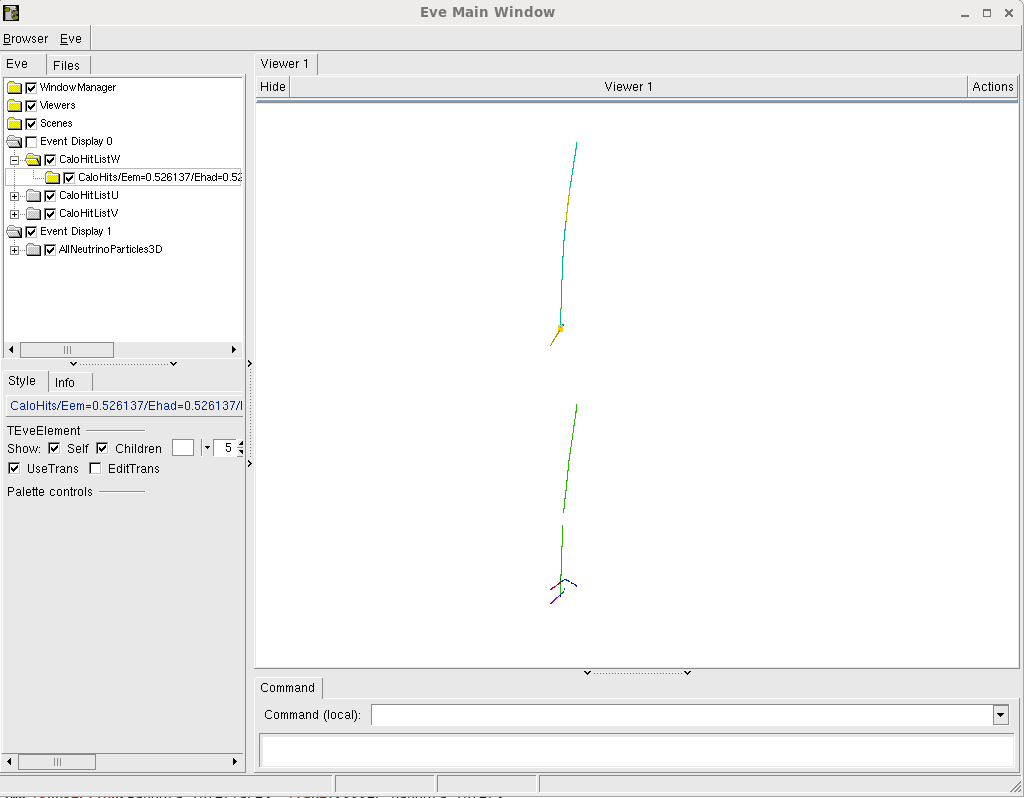
\includegraphics[width=0.5\textwidth]{/var/clus/usera/sv408/pandora_script/pandora_2}}
\centering
\caption{Pandora interface at second stage of reconstruction}
\label{fig:pandora2}
\end{figure}

\section{Write Events in Pandora Format} \label{sssec:intro}

Pandora uses special input objects (Hits, MCParticles, Gasps etc.). Those objects are already present in the .root file, but these files tends to come in a big size and for our pourposes we do not need all the information they contain. For this reason, it is possible to serialise input objects in .pndr files (which are small, but the portability is not guaranteed) or .xml files (which are large, but compressible). First thing to do is downloading a new .xml file which will give the command to write a .pndr file.

\begin{verbatim}

cp $LARPANDORA_DIR/scripts/PandoraSettings_Write.xml ./MyPandoraSettings_Write.xml

\end{verbatim} 

The file will be the following:

\begin{lstlisting}[language=XML, caption=Python example]

<!-- Pandora settings xml file -->

<pandora>
    <!-- GLOBAL SETTINGS -->
    <IsMonitoringEnabled>false</IsMonitoringEnabled>
    <ShouldDisplayAlgorithmInfo>false</ShouldDisplayAlgorithmInfo>
    <SingleHitTypeClusteringMode>true</SingleHitTypeClusteringMode>

    <!-- PLUGIN SETTINGS -->
    <MuonPlugin>LArMuonId</MuonPlugin>

    <!-- ALGORITHM SETTINGS -->
    <!--algorithm type = "LArEventReading">
        <EventFileName>INPUT_XML_OR_PNDR_FILE</EventFileName>
        <ShouldReadEvents>true</ShouldReadEvents>
        <SkipToEvent>0</SkipToEvent>
    </algorithm-->

     <algorithm type = "LArEventWriting">
        <EventFileName>Pandora_Events.pndr</EventFileName>
        <ShouldWriteEvents>true</ShouldWriteEvents>
        <ShouldOverwriteEventFile>true</ShouldOverwriteEventFile>
        <ShouldWriteMCRelationships>true</ShouldWriteMCRelationships>
        <ShouldWriteTrackRelationships>true</ShouldWriteTrackRelationships>
    </algorithm>
</pandora>

\end{lstlisting}

edit line 20 as it follows, if for example you want as an output the file "MyPandoraEvents.pndr":

\begin{verbatim}

<EventFileName>MyPandoraEvents.pndr</EventFileName>

\end{verbatim}

Then modify myreco${\_}$uboone${\_}$mcc7${\_}$driver${\_}$stage2.fcl as well:

\begin{verbatim}

physics.reco: [ pandoraNu, pandoraWriter]

\end{verbatim}

At this point, launch

\begin{verbatim}

lar -c myreco_uboone_mcc7_driver_stage2.fcl -n 5 /path/to/reco2/file.root 

\end{verbatim}

and in your folder the file MyPandoraEvents.pndr will be created.
%\afterpage{\null\newpage}
